\let\textcircled=\pgftextcircled
\chapter{Concepts généraux}
\label{chap:background}
%\mtcaddchapter
%\adjustmtc

\initial{D}\textit{ans ce chapitre nous introduisons ou rappelons les informations et concepts de base nécessaires à la compréhension du travail présenté dans ce document. Il s'agit des notions liées à la \textbf{virtualisation} et au \textbf{PML}.}

%\minitoc

\newpage    
%%%%%%%%%%%%%%%%%%%%%%%%%SECTION VIRTUALISATION%%%%%%%%%%%%%%%%%%%%%%%%%%%%%%%%%%%%%%%%%%%%%%%%%%%%%%%%%
\section{Généralités sur la Virtualisation}

\subsection{Définition}
\par\noindent La virtualisation est l’ensemble des techniques matérielles ou logicielles qui permettent de faire fonctionner simultanément sur une seule machine physique (machine hôte) plusieurs systèmes d’exploitation (\textit{\acs{OS} : \acl{OS}}) appelés \ac{VMs} (\textit{Virtual Machines, en anglais}). L'architecture d'un environnement virtualisé est présentée par la figure \ref{fig:environnement_virtualise} suivante :\\

\begin{figure}[H]
    \centering
    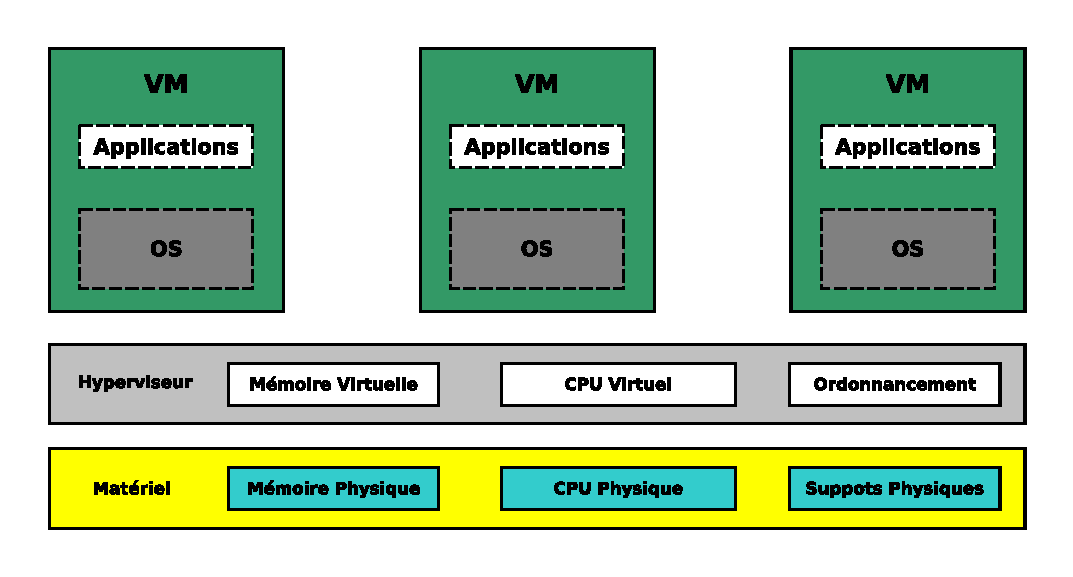
\includegraphics[scale=.7]{chapters/1/fig1/environnement_virtualise}
    \caption{Architecture d'un système virtualisé}
    \label{fig:environnement_virtualise}
\end{figure}

\par\noindent La plupart des serveurs (non virtualisés) utilisent moins de 15\% de leurs capacités \cite{online1}, ce qui favorise leur prolifération et la complexité de leur gestion. La virtualisation résout ces problèmes d’efficacité en permettant l'exécution de plusieurs systèmes d’exploitation sur un même serveur physique sous la forme de machines virtuelles, dont chacune peut accéder aux ressources de calcul du serveur sous-jacent. Chaque VM est une entité isolée, autonome et complètement indépendante des autres. Dans ces environnements virtualisés, un système de virtualisation, \ac{VMM}, est responsable de la gestion de ces machines virtuelles et du partage des ressources entre elles. Il émule le matériel pour elles, et établit la communication entre elles et les périphériques (de la machine hôte). Il existe plusieurs techniques de virtualisation.

\subsection{Techniques de virtualisation}
En fonction de la position du système de virtualisation et des machines virtuelles par rapport au matériel, il existe cinq techniques de virtualisation:

\subsubsection{Virtualisation niveau OS ou isolation}
Cette technique de virtualisation permet d'isoler l'exécution des applications des zones d'exécution appelées contextes ou containers. Ici, l'\acs{OS} hôte dispose des mécanismes pour construire des containers isolés (VMs). Ces derniers partagent le même OS (l'hôte). La \ac{VMM} fait donc partie de l'OS hôte. Cette solution est très bonne en performance, mais les environnements virtualisés ne sont pas complètement isolés. La figure \ref{fig:virtualisation_niveau_os} présente l'architecture de cette technique de virtualisation.
    
    \begin{figure}[H]
      \centering
      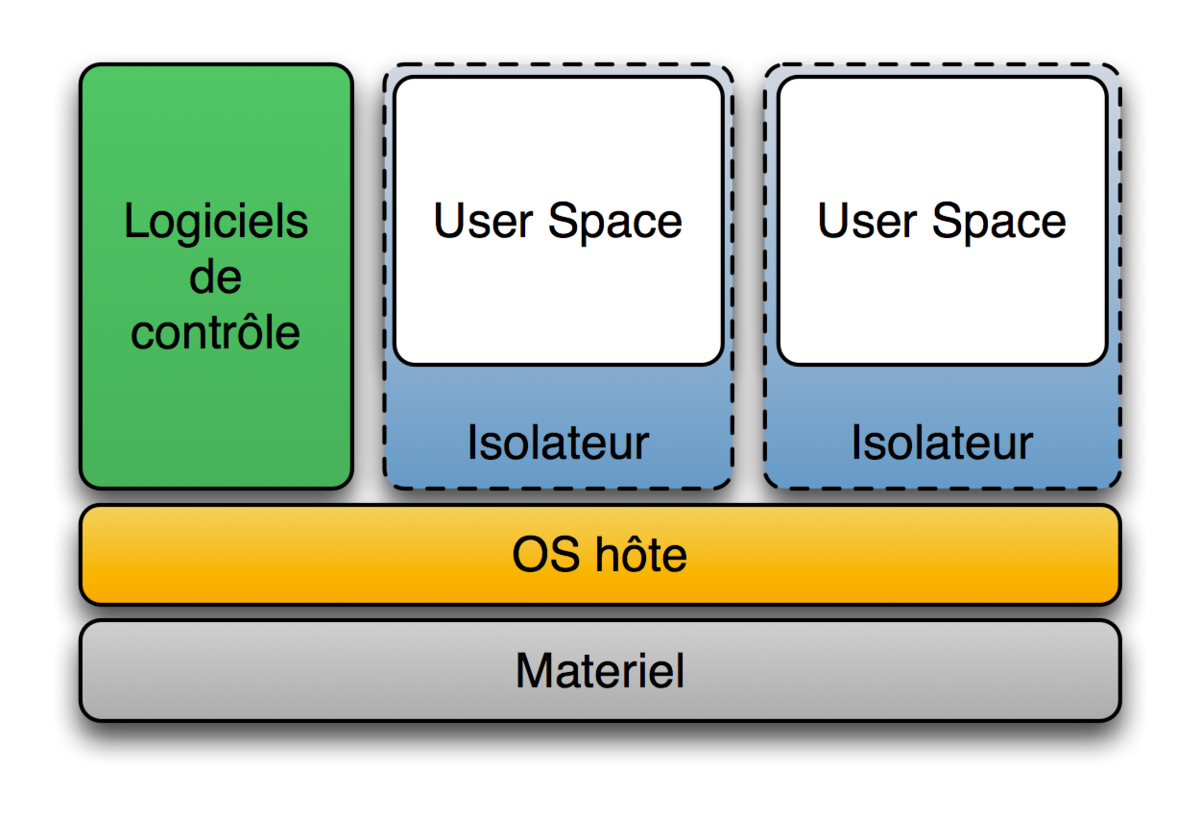
\includegraphics[scale=.8]{fig1/virtualisation_niveau_os.png}
      \caption{Architecture Virtualisation niveau OS}
      \label{fig:virtualisation_niveau_os}
      %\vspace{10px}
      \centering \bfseries Source : référence \cite{online2}
    \end{figure}
    
\noindent \textbf{Exemples :} OpenVZ,  BSD Jail, chroot, Linux-VServer, Linux containers.
    
\subsubsection{Noyau en espace utilisateur}
Un noyau en espace utilisateur (user-space) tourne comme une application en espace utilisateur de l'OS hôte. Le noyau user-space a donc son propre espace utilisateur dans lequel il contrôle ses applications. Cette solution est très peu performante, car deux noyaux sont empilés, l’isolation des environnements n’est pas gérée et l’indépendance par rapport au système hôte est inexistante. Elle sert surtout au développement du noyau. La figure \ref{fig:noyau_espace_utilisateur} présente l'architecture de cette technique de virtualisation.
    \begin{figure}[H]
      \centering
      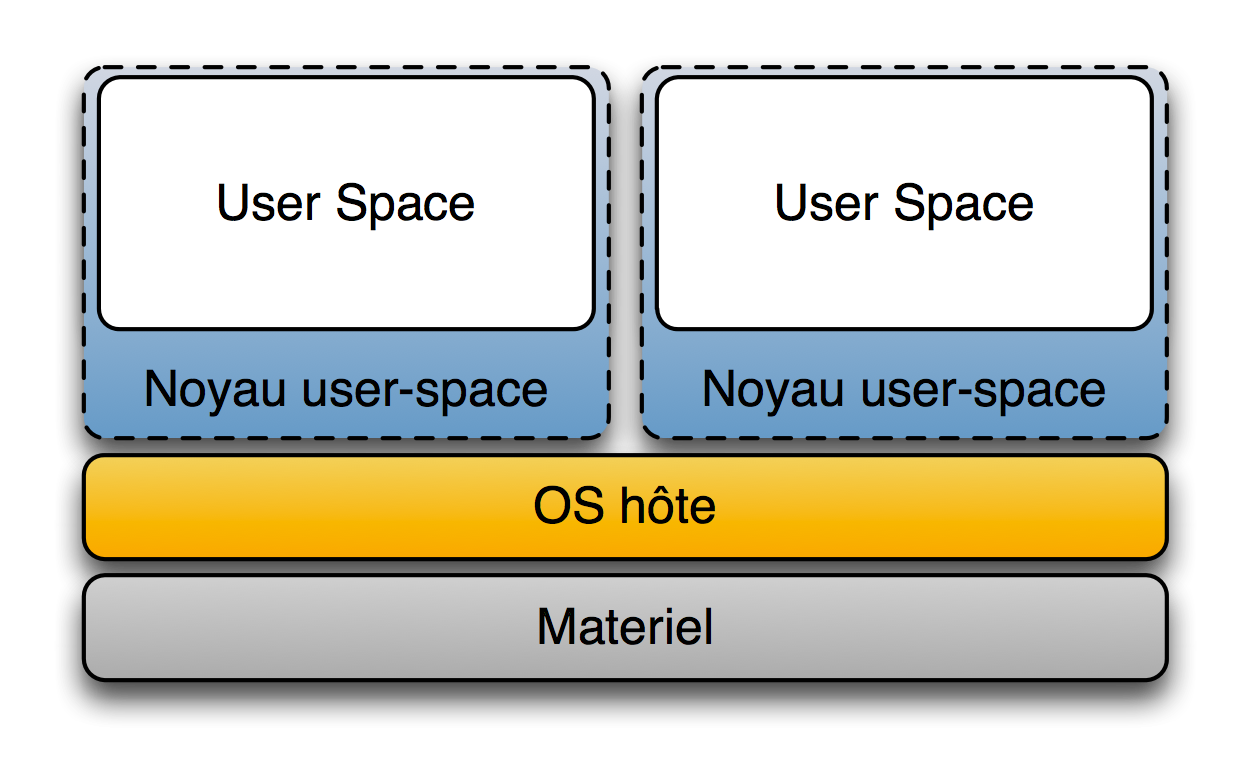
\includegraphics[scale=.8]{fig1/noyau_espace_utilisateur.png}
      \caption{Architecture Noyau en espace utilisateur}
      \label{fig:noyau_espace_utilisateur}
      %\vspace{10px}
      \centering \bfseries Source : référence \cite{online2}
    \end{figure}
\noindent \textbf{Exemples :} User Mode Linux, Cooperative Linux, Adeos, L4Linux.
    
\subsubsection{Virtualisation complète}
Ici, un OS de base exécute des logiciels parmi lesquels la VMM, qui à son tour exécute des VMs dans l'espace utilisateur. 

\begin{figure}[H]
      \centering
      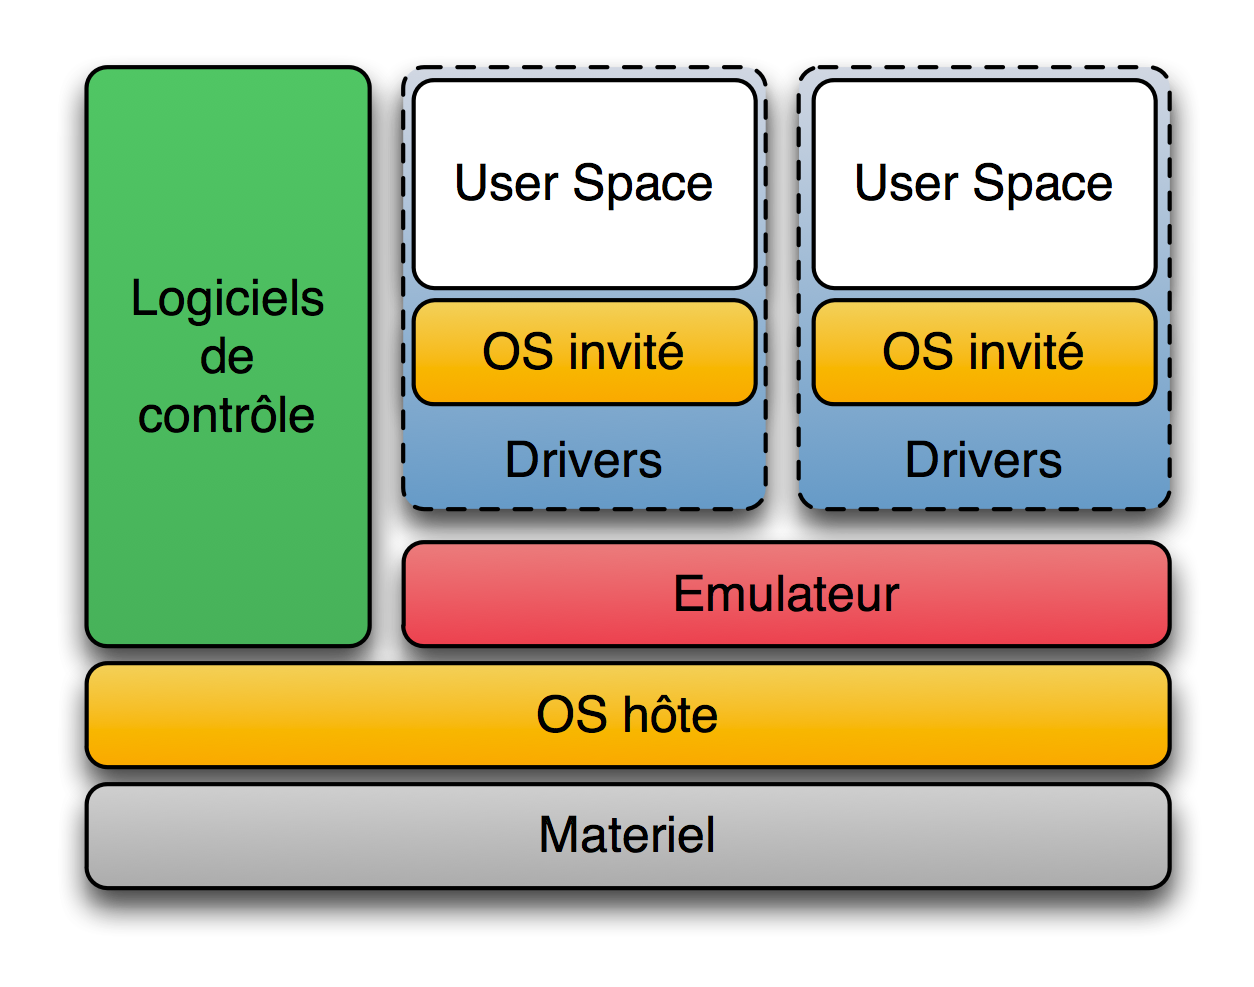
\includegraphics[scale=.8]{fig1/virtualisation_complete.png}
      \caption{Architecture Virtualisation complète}
      \label{fig:virualisation_complete}
      %\vspace{10px}
      \centering \bfseries Source : référence \cite{online2}
\end{figure}

\noindent La VMM émule le matériel pour les OS invités de façon à ce que ces derniers croient communiquer directement avec ledit matériel. L'OS de la VM est non modifié et peut être de n'importe quel type (Linux, Windows, etc.). Cette solution isole bien les OS invités, mais elle a un coût en performance qui peut être très élevé.  La figure \ref{fig:virualisation_complete} présente l'architecture de cette technique de virtualisation.\\

\noindent \textbf{Exemples :} Oracle VM VirtualBox, QEMU, KVM, Microsoft VirtualPC, VMware Workstation.

\subsubsection{Para-virtualisation}
La VMM (ici appelée hyperviseur) remplace l'OS hôte et sert d'intermédiaire pour communiquer avec le matériel. Les OS invités fonctionnent en ayant conscience d'être virtualisés et sont optimisés pour ce fait. L'OS hôte est lui-même considéré comme une VM (privilégiée) et est utilisé par la VMM pour assurer certaines tâches. C'est la méthode de virtualisation la plus performante, mais elle a pour contrainte d'exiger la modification des OS des VMs. La figure \ref{fig:para_virtualisation} présente l'architecture de cette technique de virtualisation.

\begin{figure}[H]
      \centering
      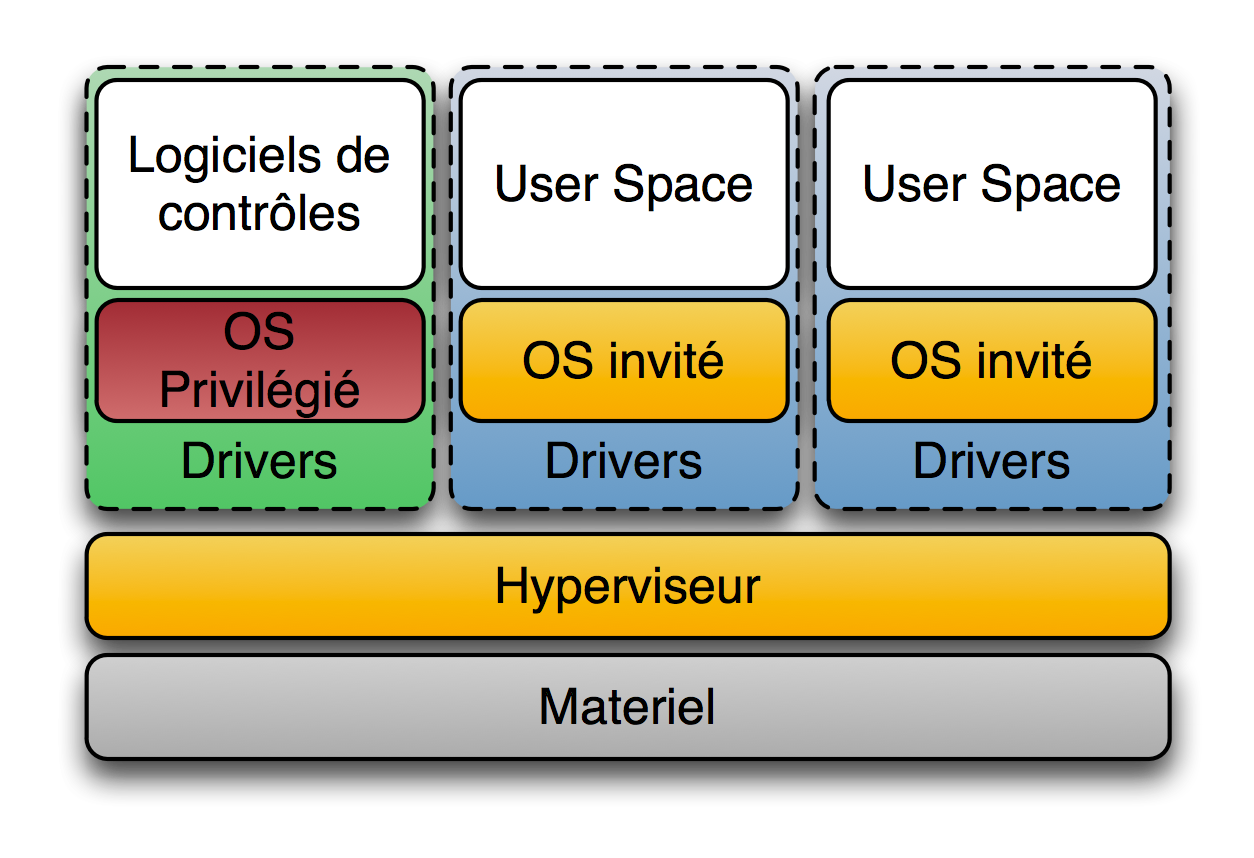
\includegraphics[scale=.8]{fig1/para_virtualisation.png}
      \caption{Architecture Para-virtualisation}
      \label{fig:para_virtualisation}
      %\vspace{10px}
      \centering \bfseries Source : référence \cite{online2}
\end{figure}

\noindent \textbf{Exemples :} Xen, VMware vSphere,  Microsoft Hyper-V Server, Parallels Server Bare Metal.
    
\subsubsection{Virtualisation assistée par le matériel}
\label{subsubsection:hvm}
C'est une sorte de para-virtualisation sans intervention de l'OS hôte et dans laquelle les OS des VMs ne sont plus modifiés. Ici, le matériel est au courant de la virtualisation et se charge, par exemple, de virtualiser les accès mémoire ou de protéger le processeur physique des accès les plus bas niveaux. La collaboration du matériel permet de simplifier la virtualisation logicielle et de réduire la dégradation de performances. En outre, ici les VMs portent le nom de \ac{HVM}.
    \\ \textbf{Exemples :} AMD-V (assistance à la virtualisation de AMD) et Intel VT (assistance à la virtualisation de Intel).

%\begin{landscape}
\begin{comment}
\newcommand{\hauteurgraphiques}{6cm}
\begin{figure}[H]
    \begin{minipage}{0.49\textwidth}
        \centering
        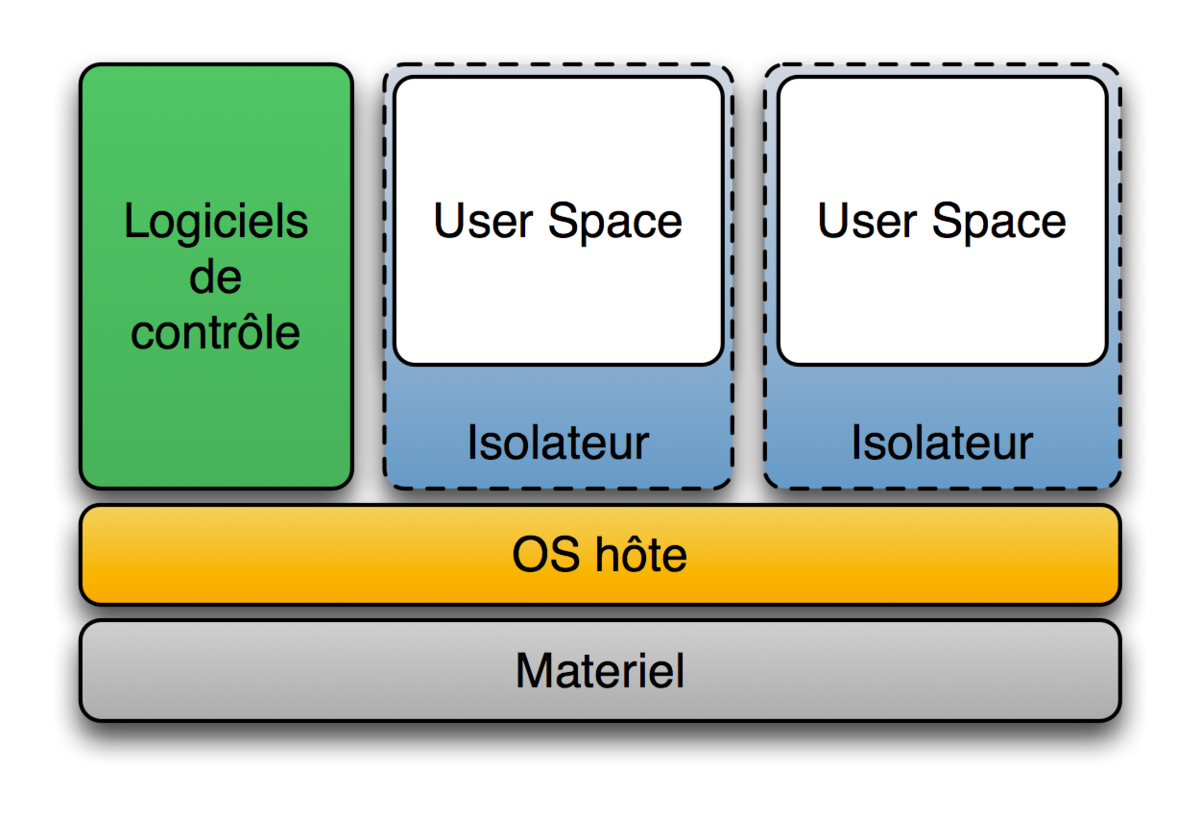
\includegraphics[width=1\linewidth,height=\hauteurgraphiques]{fig1/virtualisation_niveau_os.png}
        \caption{Architecture Virtualisation niveau OS}
        \label{fig:virtualisation_niveau_os}
    \end{minipage}
    \hspace{\fill}
    \begin{minipage}{0.49\textwidth}
        \centering
        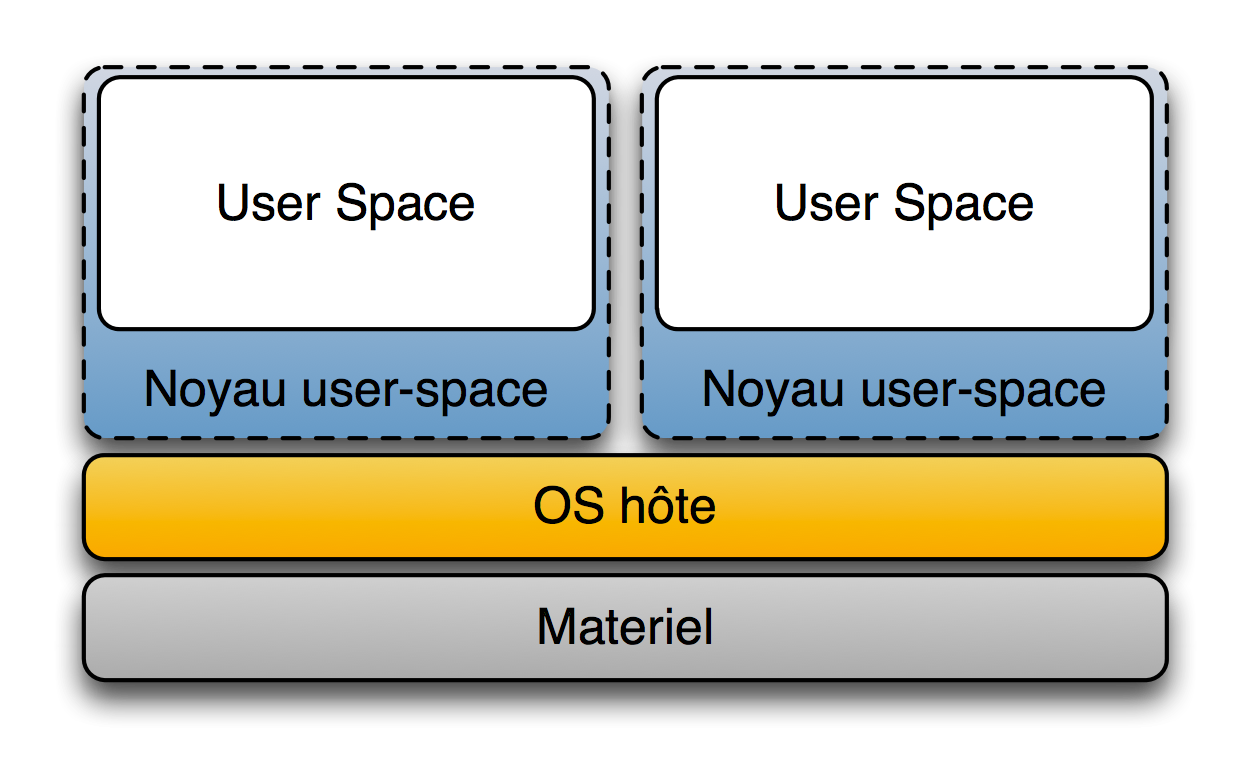
\includegraphics[width=1\linewidth,height=\hauteurgraphiques]{fig1/noyau_espace_utilisateur.png}
        \caption{Architecture Noyau en espace utilisateur}
        \label{fig:noyau_espace_utilisateur}
    \end{minipage}
    \begin{minipage}{0.49\textwidth}
        \centering
        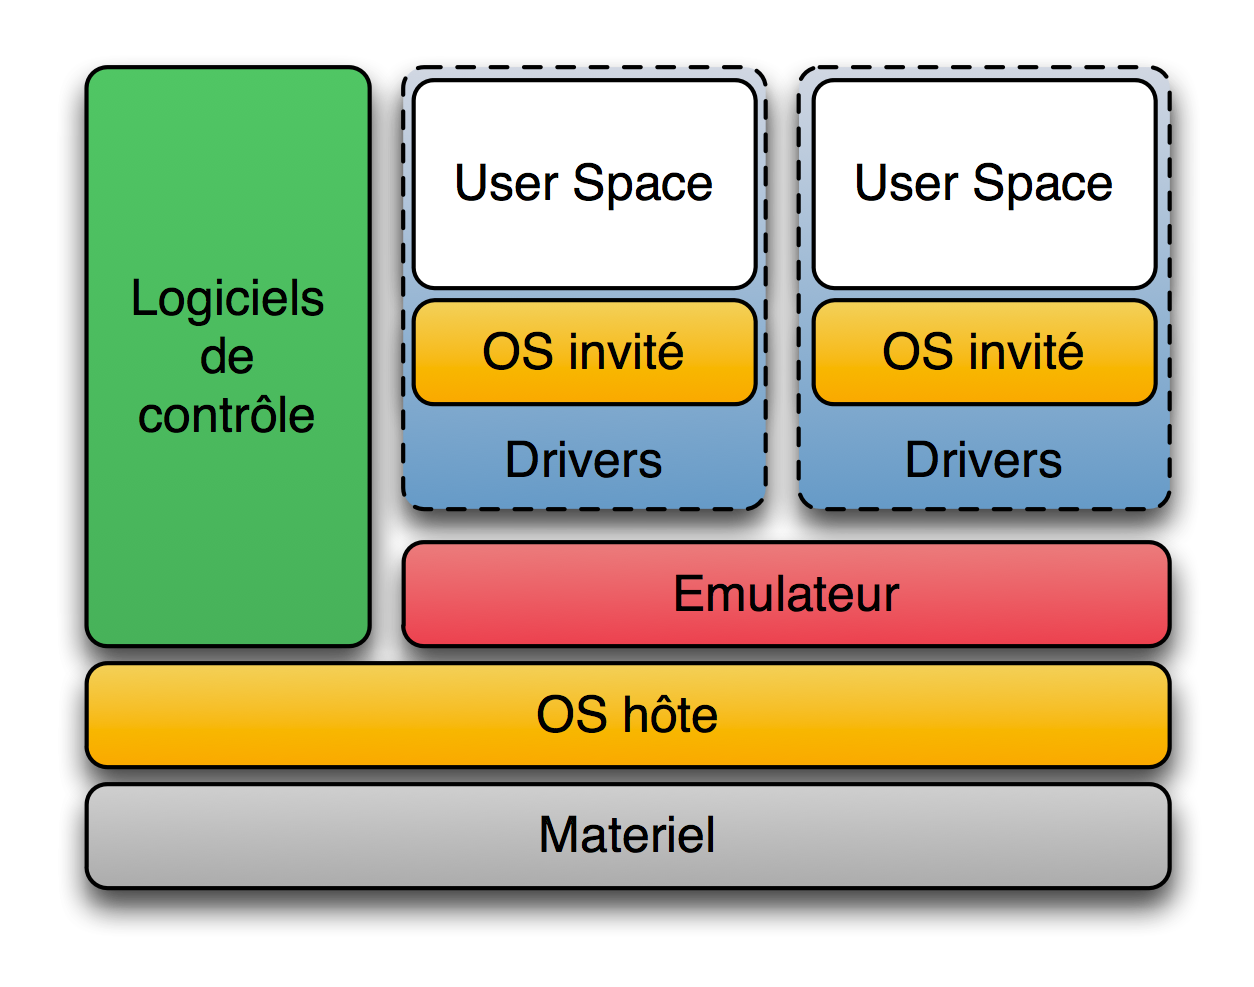
\includegraphics[width=1\linewidth,height=\hauteurgraphiques]{fig1/virtualisation_complete.png}
        \caption{Architecture Virtualisation complète}
        \label{fig:virualisation_complete}
    \end{minipage}
    \hspace{\fill}
    \begin{minipage}{0.49\textwidth}
        \centering
        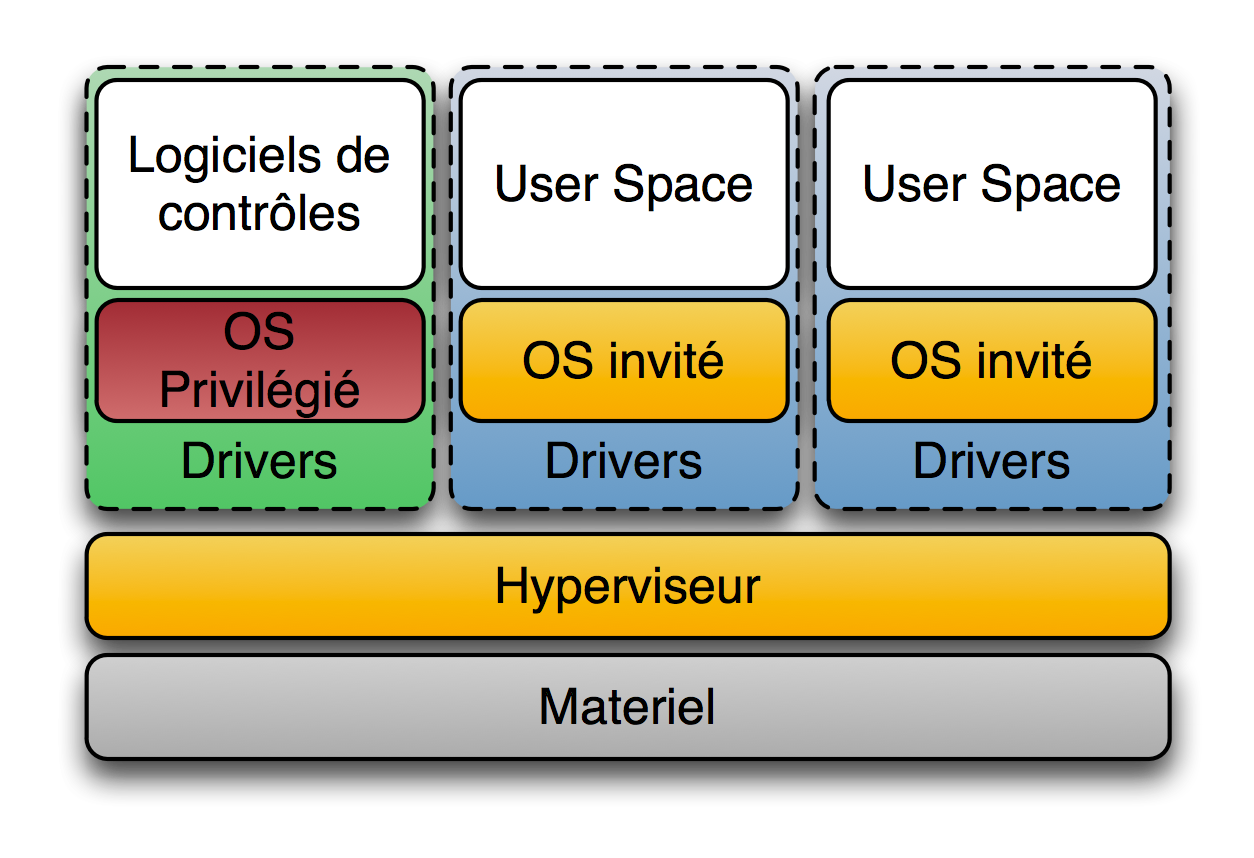
\includegraphics[width=1\linewidth,height=\hauteurgraphiques]{fig1/para_virtualisation.png}
        \caption{Architecture Para-virtualisation}
        \label{fig:para_virtualisation}
    \end{minipage}
    \vspace{20px}
    \centering \bfseries Source des images: \cite{online2}
\end{figure}
%\end{landscape}
\end{comment}

\subsection{Systèmes de virtualisation}
Le tableau suivant (\ref{tab:sytemes_virtualisation}) récapitule certaines \acs{VMM}s en fonction de leur type de virtualisation :
\begin{table}[H]
  \begin{center}
    \caption{Systèmes de virtualisation en fonction du type de virtualisation}
    \begin{tabular}{>{\bfseries}l r}
      \hline
      \textbf{VMM} & \textbf{Technique de virtualisation} \\
      \hline
      OpenVZ & Niveau OS \\ 
      Linux-VServer & Niveau OS \\ 
      L4Linux & Noyau en espace utilisateur \\ 
      Adeos & Noyau en espace utilisateur \\ 
      Oracle VM Virtualbox & Virtualisation complète \\
      QEMU & Virtualisation complète \\ 
      VMWare vSphere & Para-virtualisation \\ 
      Xen & Para-virtualisation \\   \hline
    \end{tabular}
    \label{tab:sytemes_virtualisation}
  \end{center}
\end{table}

\noindent Le système que nous utilisons dans le cadre de ce travail est \textbf{XEN}. \emph{XEN} est un système de virtualisation assez connu \cite{article2} et utilisé par Amazon pour virtualiser ses datacenters\cite{online4}. Il s'appuie sur un hyperviseur qui s'exécute sur le matériel et une machine virtuelle particulière appelée \textit{\textbf{dom0}} : il s'agit de l'OS de la machine hôte. Les services de l'OS hôte ne sont pas inclus dans l'hyperviseur afin de le maintenir aussi léger que possible. Les autres VMs ici sont appelées \textit{\textbf{domU}} (voir figure \ref{fig:virtualisation_xen}).\\

\begin{figure}[H]
      \centering
      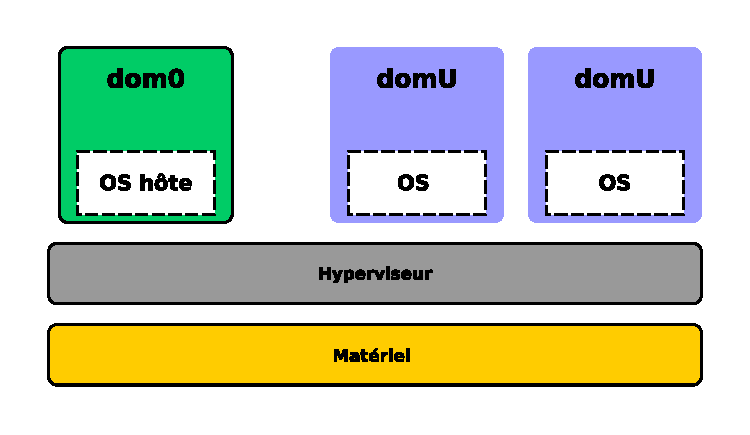
\includegraphics[scale=.7]{fig1/virtualisation_xen}
      \caption{Architecture Virtualisation avec hyperviseur XEN}
      \label{fig:virtualisation_xen}
\end{figure}

\subsection{Avantages de la virtualisation}
Selon le dernier rapport de l’entreprise de conseil et de recherche Gartner Inc. au sujet de la virtualisation, le niveau de pénétration de la virtualisation est assez élevé, avec plusieurs organisations ayant un taux de virtualisation de leurs serveurs excédant les 75\% \cite{online3}. Cette utilisation de plus en plus importante des techniques de virtualisation dans les DCs doit son mérite aux nombreux avantages qu'elles offrent. Ceux-ci sont relatifs à :

\begin{itemize}[label=\ding{42}, font=\large \color{darkorange}]
    \item \textbf{La réduction des coûts} : le fait que plusieurs VMs peuvent s'exécuter sur une même machine hôte entraîne une réduction du nombre de serveurs physiques et donc une réduction des coûts liés à l'acquisition, l'exploitation et l'expansion de l'infrastructure. 
    \item \textbf{L'isolation et l'amélioration de la sécurité} : la virtualisation offre la possibilité de séparer les différentes tâches d'un serveur physique entre plusieurs VMs, ce qui permet donc de les isoler les unes des autres et donc d'accroître le niveau de sécurité.
    \item \textbf{La minimisation des interruptions et l'amélioration de la disponibilité des services} : les solutions de virtualisation rendent possible la migration de machines virtuelles d'un serveur physique à un autre \cite{article3, article4}. Cette fonctionnalité est un élément important qui améliore la disponibilité des services.
    \item \textbf{L'optimisation des performances} : un autre avantage de la migration de machines virtuelles est qu'elle rend possible de distribuer les charges de travail entre les différents serveurs physiques \cite{article3, article4}. Ceci permet donc une meilleure gestion des ressources et donc une optimatisation des performances.
    \item \textbf{La simplification des opérations de sauvegarde} : qui améliore la tolérance aux pannes.
\end{itemize}

\section{Virtualisation de la mémoire}
Bien que la virtualisation présente de nombreux avantages, les coûts qu'elle engendre (surcharge des processeurs, etc.) ne sont pas négligeables. L'une des sources majeures de ces coûts de performance dans les environnements virtualisés c'est la virtualisation de la mémoire, à travers la traduction d'adresses \cite{article6, article8}. En effet, les adresses des processus qui s'exécutent dans les VMs ne sont pas des adresses de la mémoire \textit{réelle} (dans le système hôte), mais des adresses virtuelles, qui doivent être traduites en adresses physiques dans la mémoire centrale. 

\subsection{Environnement natif (sans virtualisation)}
Dans un environnement natif, les adresses utilisées par un processus (ou application) sont des adresses virtuelles (Vaddr, pour \textit{virtual address}). Chaque processus maintient une table de pages qui contient les correspondances entre ces adresses et les adresses physiques correspondantes (voir figure \ref{fig:vaddr_paddr_natif}).

\begin{figure}[H]
    \centering
    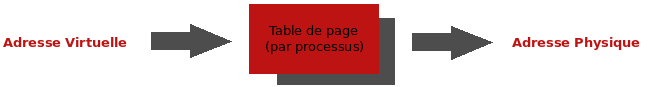
\includegraphics[scale=.65]{chapters/1/fig1/vaddr_paddr}
    \caption{Translation adresse virtuelle - adresse physique (environnement natif)}
    \label{fig:vaddr_paddr_natif}
\end{figure}

\noindent On a donc un seul niveau de parcours de table de pages dans un environnement natif. La figure \ref{fig:parcours_1D} illustre ce parcours.

\begin{figure}[H]
    \centering
    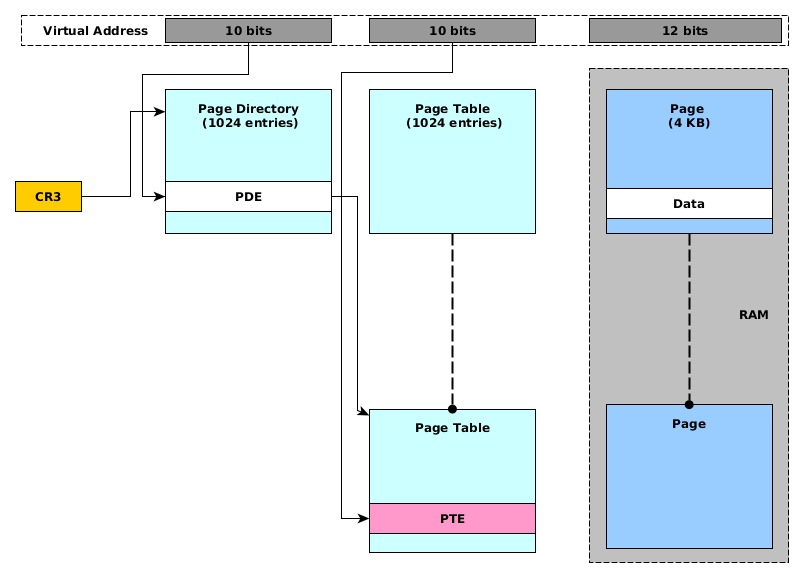
\includegraphics[scale=.55]{chapters/1/fig1/parcours_1D}
    \caption{Parcours table de page 1D (une dimension)}
    \label{fig:parcours_1D}
\end{figure}

\subsection{Environnement virtualisé}
Dans un environnement virtualisé chaque VM est un OS à part entière, donc les processus qui s'y exécutent maintiennent une table de page (\textit{\acl{gPT}, \acs{gPT}}), comme dans un environnement natif, pour effectuer la translation d'adresses virtuelles, appelées ici \ac{gVA}, en adresses physiques \textit{\textbf{\ac{gPA}}}. Ici, deux approches ou mécanismes de translation sont utilisés : \textit{\textbf{shadow paging}} et \textit{\textbf{nested paging}}.\\

\noindent Avant d'aborder ces notions, nous allons parler en quelques mots de la TLB (\textit{\acl{TLB}}). 

\subsubsection{Translation Lookaside Buffer (TLB)}
La TLB est une mémoire \textit{cache} utilisée pour réduire le temps d'accès à la mémoire centrale \cite{article7, book2}. Elle enregistre les données récentes des tables de pages, à savoir les translations d'adresses récentes \textit{\textbf{\acs{Vaddr} --> hPA}}.\\
Il existe une entrée de la table de pages pour l'intégralité de l'espace d'adressage de chaque programme. Mais étant donné que la table de pages est en mémoire centrale, cela ralentirait le processeur d'aller chercher la correspondance de chaque adresse virtuelle en mémoire centrale. Ainsi la TLB contient les données les plus récemment chargées à partir des tables de pages à l'intérieur du processeur lui-même. Si l'adresse recherchée est trouvée dans la TLB, le processeur peut directement aller à l'emplacement mémoire correspondant. Dans le cas contraire on parle de \textit{\textbf{TLB miss}}. Le processeur doit donc aller en mémoire trouver la table de pages et charger dans la TLB l'entrée de la table correspondant à l'adresse recherchée. La figure \ref{fig:tlb} présente le fonctionnement global de la TLB.
\begin{figure}[H]
    \centering
    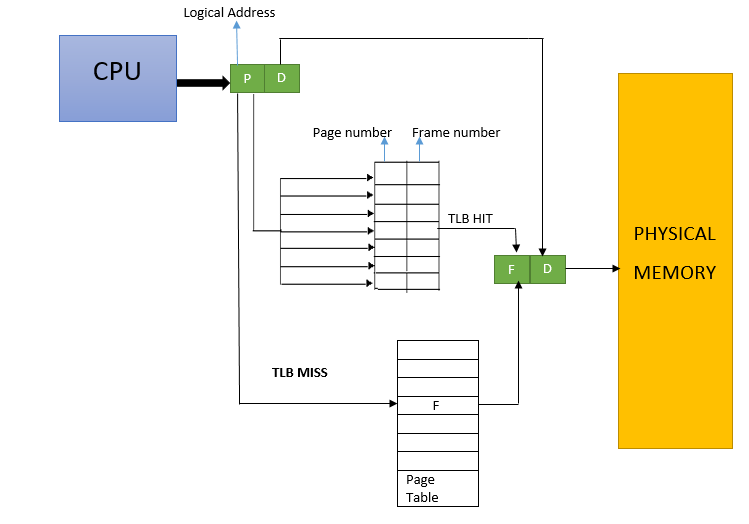
\includegraphics[scale=.7]{chapters/1/fig1/tlb}
    \caption{Fonctionnement global de la TLB}
    \label{fig:tlb}
    \centering \bfseries Source : référence\cite{tlb}
\end{figure}

\subsubsection{Shadow paging}
\label{subsubsection:shadow_paging}
\begin{enumerate}[label=\textbf{(\roman*)}]
    \item \textbf{Description}\\
    Dans cette approche, l'hyperviseur maintient une table de pages dont les entrées sont directement les correspondances \textbf{\acs{gVA} --> \acs{hPA}}. Cette table porte le nom de \textbf{\textit{shadow page table}}.\\
    A chaque tentative de la VM de mettre à jour sa table de page, l'hyperviseur capture les translations \textbf{\acs{gVA} --> \acs{gPA}} et \textbf{\acs{gPA} --> \acs{hPA}} pour construire le shadow page table. En cas de TLB miss, le processeur n'a plus qu'à effectuer un parcours 1D (une dimension) de cette table de page pour trouver l'adresse virtuelle correspondante. La figure \ref{fig:shadow} résume ce mécanisme.
    \begin{figure}[H]
        \centering
        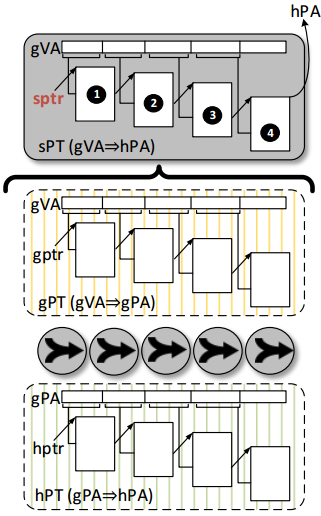
\includegraphics[scale=.6]{chapters/1/fig1/shadow}
        \caption{Mécanisme du shadow paging}
        \label{fig:shadow}
        \centering \bfseries Source : (ISCA'16 \cite{article6})
    \end{figure}
    
    \item \textbf{Avantages et Inconvénients}\\
    L'approche \textit{shadow paging}, présente les avantages suivants :
    \begin{itemize}
        \item Uniquement quatre accès mémoire requis en cas de TLB miss.
        \item Pas besoin d'un support matériel supplémentaire pour le parcours de la table de pages.
    \end{itemize}
    
    À côté de ces avantages, les points négatifs suivants sont à noter :
    \begin{itemize}
        \item Toute mise à jour de la table de pages génère une exception qui sera gérée par l'hyperviseur.
        \item Tout changement de contexte entraine des détournements coûteux dans l'hyperviseur.
    \end{itemize}
\end{enumerate}

\subsubsection{Nested paging}
\label{subsubsection:nested_paging}

\begin{figure}[H]
        \centering
        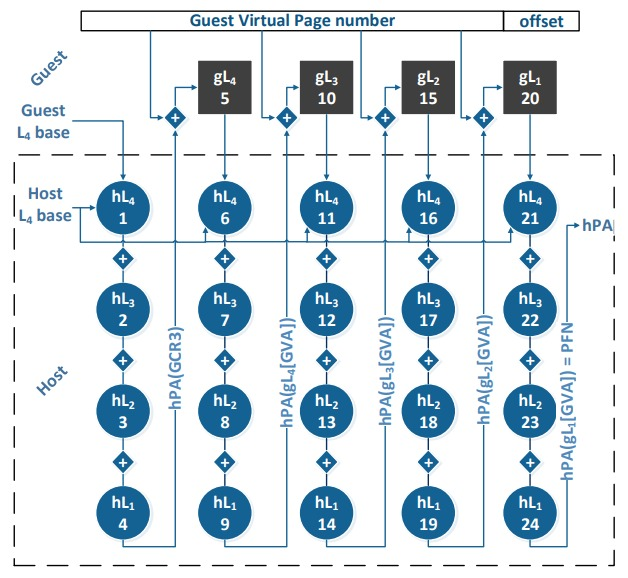
\includegraphics[scale=.5]{chapters/1/fig1/nested_paging}
        \caption{Mécanisme du nested paging}
        \label{fig:parcours_2D}
        \centering \bfseries Source : (référence \cite{article8})
\end{figure}

\begin{enumerate}[label=\textbf{(\roman*)}]
    \item \textbf{Description}\\
Cette approche est utilisée dans le cadre de la virtualisation assistée par le matériel. Ici la table de pages est imbriquée (\textit{nested}), car la translation d'adresses se fait en tenant compte de deux niveaux de table de pages : une dans la VM (\acs{gPT}), et l'autre dans l'hyperviseur. De plus, le matériel (processeur) est au courant de cette deuxième table de page dans l'hyperviseur : on parle de virtualisation complète de la mémoire.\\
Certains fabricants de processeurs ont développé des fonctionnalités pour prendre en compte cette approche de virtualisation de la mémoire :
    \begin{itemize}
        \item AMD avec le \textit{\textbf{\ac{NPT}}}
        \item Intel avec l'\textit{\textbf{\ac{EPT}}}
    \end{itemize}
    
    La figure \ref{fig:parcours_2D} décrit le parcours 2D (2 dimensions) d'une table de page imbriquée (\textit{nested page table}).

    \item \textbf{Avantages et Inconvénients}\\
    Avec cette approche, la mise à jour des tables de pages se fait rapidement et de façon directe, sans aucun détournement dans l'hyperviseur.\\
    Le principal inconvénient est le nombre d'accès mémoire nécessaires en cas de TLB miss (24 au total, voir figure \ref{fig:parcours_2D}).
\end{enumerate}

%%%%%%%%%%%%%%%%%%%%%%%%%SECTION PML%%%%%%%%%%%%%%%%%%%%%%%%%%%%%%%%%%%%%%%%%%%%%%%%%%%%%%%%%
\section{Page Modification Logging (PML)}
\subsection{Intel VT-x}
\label{subsubsection:intel_vtx}
Pour mieux comprendre ce qu'est le PML, il est nécessaire de connaître certaines notions relatives aux supports matériels des processeurs Intel pour la virtualisation.\\
Dans le cadre de la virtualisation assistée par le matériel (sous-section \ref{subsubsection:hvm}), la virtualisation s'étend à la mémoire et au processeur.  Dans la sous-section \ref{subsubsection:nested_paging}, nous avons avons fait allusion à l'EPT qui est la technologie introduite par Intel pour la virtualisation de la mémoire. En ce qui concerne la virtualisation du CPU (processeur), Intel a introduit les \acs{VT-x} (\acl{VT-x}).\\
Les extensions \acs{VT-x} dupliquent entièrement l'état architectural visible du processeur et introduisent un nouveau mode d'exécution, le \textbf{\textit{mode root}}. Ainsi, l'hyperviseur et l'\acs{OS} hôte s'exécutent en mode root (avec tous les droits et privilèges), et les autres VMs en \textit{mode no-root} (avec des accès restreints).\\
Avec les VT-x, chaque VM a une structure de données en mémoire centrale, gérée par la \acs{VMM} et appelée \textit{\textbf{\ac{VMCS}.}} Cette structure de contrôle sert à sauvegarder l'état de la VM. Lorsque l'état de la VM est chargée, cette dernière s'exécute en mode non-root jusqu'à ce qu'elle génère une exception qui doive être gérée par l'hyperviseur : cette transition (la main passe de la VM à l'hyperviseur qui doit gérer l'exception) du mode non-root au mode root est appelée \textit{\textbf{VMExit}}.

\subsection{Description du PML}
\label{subsubsection:description_pml}
Le \acs{PML} est utilisé dans le cadre de la virtualisation. C'est une amélioration de la technologie \textit{\ac{Intel VT}}. Il étend les capacités des VMM qui utilisent le mécanisme d'\acs{EPT}, en leur donnant la possibilité de traquer les pages mémoire modifiées par les \acs{VMs} (\textit{guest-physical pages}) durant leur exécution \cite{online5}.\\
Intel a inclu dans ses processeurs récents des bits \ac{A/D} \footnote{Lorsqu'un processus accède à une page mémoire, pendant la translation d'adresse lors du parcours de l'EPT, le bit \textit{accessed} correspondant est mis à 1. De même le bit \textit{dirty} est mis à 1 pour signifier que la page a été modifiée.} pour l'\acs{EPT} \cite{book3}. Etant donné que ces bits sont définis ou mis à jour sans invoquer la VMM, elle n'a aucun moyen d'accumuler des statistiques de \textit{working set} (pages utilisées, modifiées, etc.) pendant l'exécution de la VM. Pour obtenir de telles statistiques, la VMM doit scanner à tout moment l'EPT pour collecter les informations sur les bits \textit{accessed} et \textit{dirty}, ou alors marquer les pages comme \textit{non présentes} ou \emph{en lecture seule}, de sorte que si un processus tente d'accéder à une page ou de la modifier, cela génère une exception que la VMM pourra capturer. De telles opérations imposent des coûts de latence et de performance qui sont inacceptables dans certaines circonstances.

\noindent Le PML s'appuie sur la prise en charge par le processeur des bits \acs{A/D} de l'\acs{EPT} (sous-section \ref{subsubsection:nested_paging} : virtualisation complète de la mémoire). En effet, il étend le procédé qui se produit lorsque les bits \textit{dirty} sont mis à jour (quand une page mémoire est modifiée). Lorsqu'une écriture fait passer un bit \textit{dirty} de 0 à 1, le processeur enregistre l'adresse physique (\acs{gPA}) de la page mémoire\footnote{Il s'agit des \textit{guest-physical adresses}, i.e. des pages mémoire des processus s'exécutant dans la VM.} à l'origine de cet accès dans un emplacement mémoire sous le nom de \textit{page modification log}. Lorsque cette page de logs est pleine (512 entrées), le processeur génère un \textit{VMExit}. Pendant ce \textit{VMExit}, aucune adresse supplémentaire n'est enregistrée\footnote{Car pendant un VMExit, la VM est en pause étant donné que l'hyperviseur prend la main.}, et le processeur met effectivement à jour les bits dirty des adresses correspondantes dans une structure de données associée à chaque VM et appelée \emph{bitmap} (voir paragraphe \ref{subsection:design_actuel_pml}).\\

\par\noindent L'introduction du PML a nécessité des changements spécifiques dans les \acs{VMCS}
 : 
\begin{itemize}
    \item \textit{\textbf{enable PML}} : c'est le bit 17 du régistre de contrôle spécifique \textit{«secondary processor-based VMexecution control»}. Il doit être mis à 1 pour activer le mécanisme du PML (lorsqu'il est supporté par le processeur).
    \item \textit{\textbf{Page modification log}} : c'est l'espace mémoire dans lequel sont enregistrées les \acs{gPA}. Cette page comprend 512 entrées de 64 bits.
    \item \textit{\textbf{PML address}} : c'est un nouveau champ de 64 bits dans le régistre de contrôle spécifique \textit{«secondary processor-based VM execution control»}. Il représente l'adresse physique \footnote{Page mémoire de 4-KBytes} du \textit{page modification log}.
    \item \textit{\textbf{PML index}} : c'est également un nouveau champ, de 16 bits. Il représente l'index de la prochaine entrée dans le \textit{page modification log}. Etant donné que le \textit{page modification log} n'enregistre que 512 entrées, la valeur de cet index est compris entre 0 et 511.
\end{itemize}

\par\noindent Dans ce chapitre, il a été question tout d'abord d'introduire des généralités sur la \break virtualisation (les types et techniques de virtualisation), puis de parler de la vitualisation de la mémoire (en évoquant les notions de TLB, \emph{shadow} et \emph{nested} paging) et enfin d'introduire la notion de PML.